
\section{Metode Taylor\label{sec:TaylorMethods}\index{metode Taylor}\index{metode!Taylor|see {metode Taylor}}}

Solusi eksak bagi masalah nilai awal 
\begin{eqnarray}
\dot{y} & = & -\frac{y}{t}+t^{2}\nonumber \\
y(4) & = & 20\label{eq:sampleODE}
\end{eqnarray}
adalah $y(t)=\frac{t^{3}}{4}+\frac{16}{t}$, $t>0$, sebagaimana diverifikasi
dalam latihan \ref{exc:odePendulum-10} \vpageref{exc:odePendulum-10}.
Untuk sementara, mari kita mencoba melupakan bahwa kita mengetahui
solusi eksaknya, dan mempelajari metode untuk mengaproksimasinya.
Kita akan mengingat kembali bahwa kita memiliki solusi eksak ketika
tiba saatnya memeriksa perkembangan aproksimasi tersebut. Kondisi
awal, $y(4)=20$, berarti grafik solusi eksak melalui $(4,20)$. Alangkah
baiknya memulai solusi aproksimasi---pada titik yang terletak di
grafik solusi eksak! Dengan demikian, aproksimasi tersebut dimulai
dari kondisi awal. Ada banyak cara untuk melanjutkan dari sana. Barangkali
cara paling sederhana adalah menggunakan persamaan diferensial untuk
menghitung kemiringan eksak (turunan) dari $y$ pada $(4,20)$:
\begin{eqnarray*}
\dot{y}(4) & = & -\frac{y(4)}{4}+4^{2}\\
 & = & -\frac{20}{4}+4^{2}\\
 & = & 11.
\end{eqnarray*}
Anda dapat membayangkan grafik seperti itu dalam Gambar \ref{fig:numericalODE01}.
\begin{figure}
\caption{\label{fig:numericalODE01}Memulai solusi numerik dengan kondisi awal}

\begin{centering}
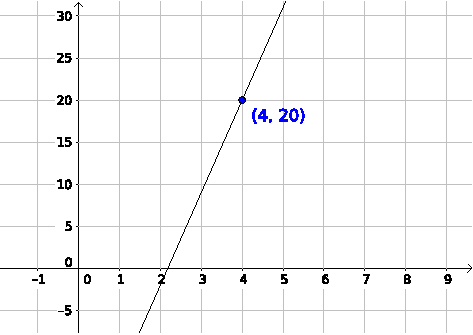
\includegraphics{figures/ode-taylor01}
\par\end{centering}
\end{figure}
 Grafik tersebut merupakan grafik polinomial Taylor orde pertama yang
dikembangkan di sekitar $t_{0}=4$. Menurut teorema Taylor, $y(t)=20+11(t-4)+\frac{\ddot{y}(\xi)}{2}(t-4)^{2}$
untuk $t$ di dekat 4 dan suatu $\xi$, yang bergantung pada $t$.
Jadi, $y(2)\approx T_{1}(2)=20+11(2-4)=-2$ dan $y(5)\approx T_{1}(5)=20+11(5-4)=31$
(selama $y$ memiliki dua turunan pada selang terbuka yang memuat
$[2,5]$), dan seterusnya. Seperti biasa, ada kekhawatiran mengenai
seberapa baik aproksimasi ini.

Dalam bagian \ref{sec:Composite}, dua aproksimasi berbeda untuk bilangan
yang sama digunakan untuk menaksir galat dalam metode adaptif. Pendekatan
serupa dapat digunakan di sini. Kita akan membandingkan aproksimasi
yang diberikan oleh $T_{1}$ dan $T_{2}$. Persamaan diferensial dapat
digunakan untuk menghitung $\ddot{y}$, dalam bentuk $y$ dan $t$.
Mendiferensialkan persamaan diferensial secara implisit menghasilkan
\[
\ddot{y}=-\frac{\dot{y}t-y}{t^{2}}+2t.
\]
Namun $\dot{y}=-\frac{y}{t}+t^{2}$, sehingga kita dapat menyubstitusikannya
dan menyederhanakan bentuk $\ddot{y}$:
\begin{eqnarray*}
\ddot{y} & = & -\frac{(-\frac{y}{t}+t^{2})t-y}{t^{2}}+2t\\
 & = & -\frac{-y+t^{3}-y}{t^{2}}+2t\\
 & = & \frac{2y}{t^{2}}-\frac{t^{3}}{t^{2}}+2t\\
 & = & \frac{2y}{t^{2}}+t.
\end{eqnarray*}
Sekarang kita mengetahui $\ddot{y}(4)=\frac{2y(4)}{4^{2}}+4=\frac{2(20)}{16}+4=\frac{13}{2}$,
sehingga $T_{2}(t)=20+11(t-4)+\frac{13}{4}(t-4)^{2}$. Akhirnya, kita
dapat membandingkan nilai $T_{1}$ dengan nilai yang bersesuaian dari
$T_{2}$, seperti dalam Tabel \ref{tab:ode-taylor1}. 
\begin{table}
\caption{\label{tab:ode-taylor1}Perbandingan aproksimasi polinomial orde pertama
dan kedua}

\begin{centering}
\begin{tabular}{c|c|c}
$t$ & $T_{1}(t)$ & $T_{2}(t)$\tabularnewline
\hline 
2 & $-2$ & 11\tabularnewline
5 & 31 & $34.25$\tabularnewline
\end{tabular}
\par\end{centering}
\end{table}
 $T_{1}(2)$ dan $T_{2}(2)$ sangat berbeda, sehingga kita harus menganggap
bahwa kedua aproksimasi itu tidak dapat dipercaya. $T_{1}(5)$ dan
$T_{2}(5)$ hanya berbeda sekitar $10\%$, sehingga aproksimasi ini
mungkin masuk akal. Untuk semakin memperhalus aproksimasi $y(2)$,
kita dapat menghitung $T_{3}(2)$ dan membandingkannya lagi. Dapatkah
Anda melakukannya? Jawaban \vpageref{ans:T3of2}. 

Cara lain untuk mengaproksimasi $y(2)$ adalah melakukannya sedikit
lebih perlahan. Kita dapat menggunakan kondisi awal untuk terlebih
dahulu mengaproksimasi $y(3.75)$. Kemudian kita dapat menggunakan
aproksimasi ini untuk mengaproksimasi $y(3.5)$, yang selanjutnya
dapat kita gunakan untuk mengaproksimasi $y(3.25)$, dan seterusnya
hingga akhirnya kita menggunakan aproksimasi $y(2.25)$ untuk mengaproksimasi
$y(2)$. Bagi kita manusia, melakukan semua perhitungan ini mungkin
terasa menjengkelkan, tetapi dengan sedikit kode Octave, beban itu
diserahkan kepada mesin. Kemampuan memahami proses ini dengan cukup
baik untuk menulis kode Octave itulah yang kini menjadi fokus.

Kita mengetahui bahwa $y(4)=20$ dan ingin mengaproksimasi $y(3.75)$.
Karena selisih antara $4$ dan $3.75$ hanya $.25$, penggunaan $T_{1}$
mungkin cukup akurat. Dari sebelumnya, kita mengetahui bahwa polinomial
Taylor yang dikembangkan di sekitar $t_{0}=4$ adalah $T_{1}(t)=20+11(t-4)$,
sehingga $T_{1}(3.75)=20+11(-.25)=17.25$. Sekarang kita dapat menggunakan
$y(3.75)=17.25$ sebagai kondisi awal ``baru''. $\dot{y}(3.75)=-\frac{17.25}{3.75}+3.75^{2}=9.4625$.
Kita dapat menggunakan informasi ini untuk mengaproksimasi polinomial
Taylor bagi $y$ yang dikembangkan di sekitar $3.75$: $T_{1}(t)\approx17.25+9.4625(t-3.75)$,
dan menggunakan pengembangan ini untuk mengaproksimasi $y(3.5)$:
$y(3.5)\approx T_{1}(3.5)\approx17.25+9.4625(3.5-3.75)=14.884375$.
Selanjutnya, kita dapat menggunakan $y(3.5)=14.884375$ sebagai kondisi
awal, dengan mengaproksimasi polinomial Taylor bagi $y$ yang dikembangkan
di sekitar $3.5$. Melanjutkan cara ini menghasilkan hasil tabel dan
grafik dalam Gambar \ref{fig:Euler's method}. Dapatkah Anda mereproduksi
hasil tersebut? Rincian \vpageref{ans:details}.
\begin{figure}
\caption{\label{fig:Euler's method}Perhitungan numerik berulang (dipotong
hingga 5 tempat desimal)}

\begin{centering}
\hfill{}%
\begin{tabular}{c|c}
$t_{0}$ & $y(t_{0})$\tabularnewline
\hline 
$4$ & $20$\tabularnewline
$3.75$ & $17.25$\tabularnewline
$3.5$ & $14.88437$\tabularnewline
$3.25$ & $12.88504$\tabularnewline
$3$ & $11.23557$\tabularnewline
$2.75$ & $9.92187$\tabularnewline
$2.5$ & $8.93323$\tabularnewline
$2.25$ & $8.26406$\tabularnewline
$2$ & $7.91666$\tabularnewline
\end{tabular}\hfill{}\raisebox{-.5\height}{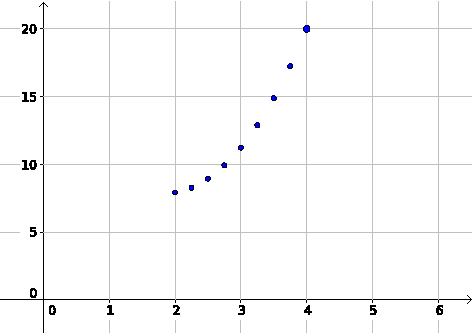
\includegraphics{figures/ode-taylor02}}\hfill{}
\par\end{centering}
\end{figure}
 

Metode perhitungan berulang menghasilkan $y(2)\approx7.91$, tetapi
yang lebih penting, memperlihatkan algoritme untuk mengaproksimasi
solusi persamaan diferensial. Dengan menyebut kondisi awal $(t_{0},y_{0})$,
dan titik-titik berikutnya $(t_{1},y_{1}),$$(t_{2},y_{2}),$$(t_{3},y_{3})\ldots$,
prosedur yang sama digunakan untuk menghitung $(t_{1},y_{1})$ dari
$(t_{0},y_{0})$ seperti yang digunakan untuk menghitung $(t_{2},y_{2})$
dari $(t_{1},y_{1})$ seperti yang digunakan untuk menghitung $(t_{3},y_{3})$
dari $(t_{2},y_{2})$, dan seterusnya. Kita tinggal menyatakan prosedur
itu dalam suatu rumus. Ringkasnya, prosedur tersebut menggunakan titik
yang diberikan, sebutlah $(t_{i},y_{i})$ untuk 
\begin{enumerate}
\item menghitung $\dot{y}(t_{i},y_{i})$;
\item menggunakan ketiga nilai $t_{i}$, $y_{i}$, dan $\dot{y}(t_{i},y_{i})$
untuk membentuk $T_{1}(t)$ yang dikembangkan di sekitar $t_{i}$;
dan akhirnya
\item menetapkan $y_{i+1}=T_{1}(t_{i+1})$, yang menghasilkan titik baru,
$(t_{i+1},y_{i+1})$.
\end{enumerate}
Namun $T_{1}(t_{i+1})=y_{i}+\dot{y}(t_{i},y_{i})\cdot(t_{i+1}-t_{i})$,
sehingga prosedur tersebut sebenarnya cukup dengan menetapkan
\begin{equation}
y_{i+1}=y_{i}+\dot{y}(t_{i},y_{i})\cdot(t_{i+1}-t_{i}).\label{eq:EulersMethodGeneral}
\end{equation}
Metode yang menggunakan rumus (\ref{eq:EulersMethodGeneral}) berulang
kali untuk menghitung barisan titik yang secara aproksimasi terletak
pada kurva solusi persamaan diferensial biasa paling sering disebut
metode Euler.\cite{butcher}\index{metode Euler}\index{metode!Euler|see {metode Euler}}
Metode ini juga dapat disebut metode Taylor berderajat 1 karena menggunakan
polinomial Taylor berderajat 1 pada setiap langkah. Nilai $t_{i+1}-t_{i}$
disebut ukuran langkah dan sering dibuat konstan, sehingga metode
Euler lazim ditulis sebagai
\begin{equation}
y_{i+1}=y_{i}+h\cdot\dot{y}(t_{i},y_{i})\label{eq:EulersMethodConstantStepSize}
\end{equation}
dengan $h=t_{i+1}-t_{i}$ adalah ukuran langkah konstan. 

\subsection{Metode Euler (kode semu)\index{metode Euler!kode semu}}

Sebagaimana lazimnya, metode Euler akan dikodekan dengan ukuran langkah
konstan.

\begin{pseudocode} 
\begin{description}
\item [{Asumsi:}] Solusi PDB ada dan tunggal pada selang dari $t_{0}$
hingga $t_{1}$.
\item [{Masukan:}] Persamaan diferensial $\dot{y}=f(t,y)$; kondisi awal
$y(t_{0})=y_{0}$; bilangan $t_{0}$ dan $t_{1}$; jumlah langkah
$N$.
\item [{Langkah\ 1:}] Tetapkan $t=t_{0}$; $y=y_{0}$; $h=(t_{1}-t_{0})/N$
\item [{Langkah~2:}] Untuk $j=1\ldots N$ lakukan Langkah 3-4:

\begin{description}
\item [{Langkah~3:}] Tetapkan $y=y+hf(t,y)$
\item [{Langkah~4:}] Tetapkan $t=t_{0}+\frac{i}{N}(t_{1}-t_{0})$
\end{description}
\item [{Keluaran:}] Nilai aproksimasi $y$ bagi solusi pada $t=t_{1}$.
\end{description}
\end{pseudocode}  

\subsection{Metode Taylor Berderajat Lebih Tinggi}

Metode Taylor berderajat lebih tinggi jarang digunakan dalam praktik
karena memerlukan perhitungan turunan, suatu tugas yang tidak selalu
mudah atau bahkan mungkin dilakukan. Meskipun demikian, mempertimbangkan
metode berderajat lebih tinggi tidaklah jauh dari apa yang telah kita
lakukan. Dengan menulis ulang langkah-langkah dalam enumerasi yang
menghasilkan \ref{eq:EulersMethodGeneral}, metode Taylor berderajat
tiga dapat diringkas sebagai
\begin{enumerate}
\item hitung $\dot{y}(t_{i},y_{i})$ \textcolor{blue}{dan $\ddot{y}(t_{i},y_{i})$
dan $\dddot{y}(t_{i},y_{i})$};
\item gunakan \textcolor{red}{\sout{tiga}} \textcolor{blue}{lima} nilai
$t_{i}$, $y_{i}$, \textcolor{red}{\sout{dan}} $\dot{y}(t_{i},y_{i})$\textcolor{blue}{,
$\ddot{y}(t_{i},y_{i})$, dan $\dddot{y}(t_{i},y_{i})$} untuk membentuk
\textcolor{red}{\sout{\mbox{$T_{1}(t)$}}} \textcolor{blue}{$T_{3}(x)$}
yang dikembangkan di sekitar $t_{i}$; dan akhirnya
\item tetapkan \textcolor{red}{\sout{\mbox{$y_{i+1}=T_{1}(t_{i+1})$}}}
${\color{blue}y_{i+1}=T_{3}(t_{i+1}}\mathclose{\color{blue})}$, yang
menghasilkan titik baru, $(t_{i+1},y_{i+1})$.
\end{enumerate}
Setelah ditulis tanpa semua penandaan, prosedurnya adalah
\begin{enumerate}
\item hitung $\dot{y}(t_{i},y_{i})$, $\ddot{y}(t_{i},y_{i})$, dan $\dddot{y}(t_{i},y_{i})$;
\item gunakan kelima nilai $t_{i}$, $y_{i}$, $\dot{y}(t_{i},y_{i})$,
$\ddot{y}(t_{i},y_{i})$, dan $\dddot{y}(t_{i},y_{i})$ untuk membentuk
$T_{3}(x)$ yang dikembangkan di sekitar $t_{i}$; dan akhirnya
\item tetapkan $y_{i+1}=T_{3}(t_{i+1})$, yang menghasilkan titik baru,
$(t_{i+1},y_{i+1})$.
\end{enumerate}
Metode Taylor berderajat lebih tinggi memerlukan turunan berorde lebih
tinggi pada langkah 1 dan polinomial Taylor berderajat lebih tinggi
pada langkah 2 dan 3. Seperti yang dapat diduga, metode berderajat
lebih tinggi umumnya lebih akurat daripada metode berderajat lebih
rendah selama rumus untuk $\dot{y}(t,y)$ cukup mulus. Untuk mengilustrasikan
hal tersebut, sekarang kita membandingkan solusi hampiran untuk \ref{eq:sampleODE}.

\subsection{Metode Taylor Berderajat 3 (Kode Semu)\index{metode Taylor berderajat 3!kode semu}}

Metode Taylor berderajat 3 akan dikodekan untuk ukuran langkah konstan.

\begin{pseudocode} 
\begin{description}
\item [{Asumsi:}] Solusi PDB ada dan tunggal pada interval dari $t_{0}$
hingga $t_{1}$.
\item [{Masukan:}] Persamaan diferensial $\dot{y}=f(t,y)$; rumus $\ddot{y}(t,y)$
dan $\dddot{y}(t,y)$; syarat awal $y(t_{0})=y_{0}$; bilangan $t_{0}$
dan $t_{1}$; jumlah langkah $N$.
\item [{Langkah\ 1:}] Tetapkan $t=t_{0}$; $y=y_{0}$; $h=(t_{1}-t_{0})/N$
\item [{Langkah~2:}] Untuk $j=1\ldots N$ lakukan Langkah 3-4:

\begin{description}
\item [{Langkah~3:}] Tetapkan $y=y+hf(t,y)+\frac{1}{2}h^{2}\ddot{y}(t,y)+\frac{1}{6}h^{3}\dddot{y}(t,y)$
\item [{Langkah~4:}] Tetapkan $t=t_{0}+\frac{i}{N}(t_{1}-t_{0})$
\end{description}
\item [{Keluaran:}] Hampiran $y$ untuk solusi pada $t=t_{1}$.
\end{description}
\end{pseudocode} 

\noindent Dengan kode Octave yang didasarkan pada kode semu yang disajikan
dalam bagian ini, Tabel \ref{tab:taylorApproximatingODE} merangkum
solusi hampiran untuk \ref{eq:sampleODE} dengan metode Euler dan
metode Taylor berderajat 3 untuk menghampiri $y(2)$.
\begin{table}
\caption{\label{tab:taylorApproximatingODE}Nilai hampiran $y(2)$ yang diperoleh
dengan menyelesaikan \ref{eq:sampleODE}}

\centering{}%
\begin{tabular}{c|cc|cc|cc|}
 & \multicolumn{1}{c|}{$h=0.5$} & galat & \multicolumn{1}{c|}{$h=0.25$} & galat & \multicolumn{1}{c|}{$h=0.125$} & galat\tabularnewline
\hline 
Metode Euler & $6.1$ & $3.9$ & $7.91666$ & $2.08333$ & $8.91911$ & $1.08088$\tabularnewline
Metode Taylor berderajat 3  & $9.975765$ & $0.024234$ & $9.996280$ & $0.003719$ & $9.999485$ & $0.000514$\tabularnewline
\end{tabular}
\end{table}

Kini saat yang tepat untuk membahas galat metode Taylor. Ingatlah
bahwa polinomial Taylor berderajat $n$ memiliki galat berorde $n+1$,
sehingga metode Euler menggunakan polinomial Taylor dengan galat berorde
2, sedangkan metode Taylor berderajat 3 menggunakan polinomial Taylor
dengan galat berorde 4. Namun, bagaimana hal tersebut tercermin dalam
suku galat \textit{metode Taylor}? 

Meskipun kita tidak akan menjawab pertanyaan ini sepenuhnya di sini,
kita dapat memperoleh gambaran tentang apa yang dapat diharapkan dari
Tabel \ref{tab:taylorApproximatingODE}. Dari baris metode Euler,
kita melihat galat berkurang dari (kira-kira) 3.9 menjadi 2.08, lalu
1.08, ketika ukuran langkah diperkecil menjadi setengahnya. Karena
\[
\frac{2.08}{3.9}\approx\frac{1.08}{2.08}\approx\left(\frac{1}{2}\right)^{1},
\]
kita menyimpulkan bahwa orde metode Euler adalah satu. Dengan meninjau
baris metode Taylor berderajat 3, kita melihat galat berkurang dari
sekitar $.024$ menjadi $.0037$ lalu $.00051$ ketika ukuran langkah
diperkecil menjadi setengahnya. Karena
\[
\frac{.0037}{.024}\approx\frac{.00051}{.0037}\approx\frac{1}{8}=\left(\frac{1}{2}\right)^{3},
\]
kita menyimpulkan bahwa orde metode Taylor berderajat 3 adalah 3.

Perhatikan kemiripan antara pengamatan ini dan pengamatan yang kita
buat mengenai integrasi komposit. Pada bagian \ref{sec:Composite},
kita berpendapat bahwa orde suku galat untuk rumus integrasi komposit
adalah satu tingkat lebih rendah daripada orde penerapan tunggal rumus
integrasi yang mendasarinya. Hal yang sama terjadi di sini. Jika galat
pemenggalan polinomial Taylor yang mendasarinya berorde $n$, metode
penyelesai PDB yang bersesuaian berorde $n-1$, yaitu orde yang sama
dengan derajat polinomial Taylor itu sendiri.

\subsection{Mereduksi persamaan orde kedua menjadi sistem orde pertama \index{persamaan diferensial!orde kedua}}

Metode Taylor dan metode Runge-Kutta yang akan dibahas semuanya dirancang
untuk menangani persamaan diferensial orde pertama. Namun, semua persamaan
gerak yang telah kita turunkan merupakan persamaan diferensial orde
kedua. Untuk mengatasi ketidaksesuaian ini, sebuah PDB orde kedua
dapat direduksi menjadi sistem orde pertama. Gagasannya sederhana.
Misalkan $y$ adalah variabel terikat dalam sebuah PDB orde kedua
dan kita memiliki persamaan berbentuk $y''=f(y',y,x)$. Kita memperkenalkan
variabel bantu $u$ dan menetapkan $u=y'$. Akibatnya, $u'=y''=f(y',y,x)=f(u,y,x)$.
Dengan demikian, kita memperoleh sistem orde pertama
\begin{eqnarray*}
u' & = & f(u,y,x)\\
y' & = & u
\end{eqnarray*}
yang dapat diselesaikan dengan metode numerik untuk persamaan diferensial
orde pertama. 

Sebagai contoh, persamaan pendulum (\ref{eq:pendulum}) dapat disusun
ulang menjadi $\ddot{\theta}=-\frac{c}{m}\dot{\theta}-\frac{g}{\ell}\sin\theta$.
Jika kita menyubstitusikan variabel bantu $u=\dot{\theta}$ ke dalam
persamaan, persamaan tersebut menjadi $\dot{u}=-\frac{c}{m}u-\frac{g}{\ell}\sin\theta$,
dan sistem 
\begin{eqnarray*}
\dot{u} & = & -\frac{c}{m}u-\frac{g}{l}\sin\theta\\
\dot{\theta} & = & u
\end{eqnarray*}
ekuivalen dengan (\ref{eq:pendulum}). Metode Euler, misalnya, dapat
diterapkan pada sistem ini dengan cara berikut:
\begin{eqnarray*}
u_{n+1} & = & u_{n}+h\left(-\frac{c}{m}u_{n}-\frac{g}{l}\sin\theta_{n}\right)\\
\theta_{n+1} & = & \theta_{n}+hu_{n}\\
t_{n+1} & = & t_{n}+h
\end{eqnarray*}
dengan $u_{0},\theta_{0},$ dan $t_{0}$ diambil dari syarat awal.

\subsection{Konsep Kunci}
\begin{description}
\item [{Metode\ Taylor:}] \index{metode Taylor}Metode untuk menghampiri
solusi sebuah PDB orde pertama yang pada setiap langkah menggunakan
polinomial Taylor dengan derajat yang telah ditentukan untuk menghitung
nilai berikutnya.
\item [{Metode\ Euler:}] \index{metode Euler}Nama lain untuk metode Taylor
orde pertama, dengan rumus $y_{i+1}=y_{i}+h\cdot\dot{y}(t_{i},y_{i})$.
\end{description}
\noindent\startexercises 

\subsection{Latihan}
\begin{enumerate}
\item \label{exc:ode-taylor}Gunakan metode Euler dengan ukuran langkah
$h=0.5$ untuk menghampiri $y(2)$.

\begin{enumerate}
\item \label{exc:ode-taylor-6} \hasasolution 
\begin{eqnarray*}
\frac{dy}{dx} & = & 3x-2y\\
y(1) & = & 1
\end{eqnarray*}
\item 
\begin{eqnarray*}
\frac{dy}{dx} & = & 3x^{3}-y\\
y(1) & = & 3
\end{eqnarray*}
\item \label{exc:ode-taylor-7} \hasananswer 
\begin{eqnarray*}
\dot{y} & = & ty\\
y(1) & = & 0.5
\end{eqnarray*}
\item \label{exc:ode-taylor-8} \hasasolution 
\begin{eqnarray*}
\cos(x)y'+\sin(x)y & = & 2\cos^{3}(x)\sin(x)-1\\
y(1) & = & 0
\end{eqnarray*}
\item 
\begin{eqnarray*}
7\dot{y}+3y & = & 5\\
y(1) & = & 2
\end{eqnarray*}
\end{enumerate}
\item \label{exc:ode-taylor-9}Ulangi latihan \ref{exc:ode-taylor} dengan
menggunakan metode Taylor orde 2.  \haspartwithsolution  \haspartwithanswer 
\item \label{exc:ode-taylor-10}Ulangi latihan \ref{exc:ode-taylor} dengan
menggunakan metode Taylor orde 3.  \haspartwithsolution  \haspartwithanswer 
\item \label{exc:ode-taylor-1}Lakukan dua langkah metode Euler untuk menyelesaikan
$\dot{y}=ty$ dengan $y(1)=-0.5$ dan $h=0.25$, sehingga diperoleh
aproksimasi $y(1.5)$. \hasananswer 
\item \label{exc:ode-taylor-11}Tulislah kode semu untuk metode Taylor orde
2. \hasananswer 
\item Tulislah kode semu untuk metode Taylor orde 4.
\item \label{exc:ode-taylor-2} \octave\ Tulislah fungsi Octave yang mengimplementasikan
metode Euler.  \hasasolution 
\item \label{exc:ode-taylor-3} \octave\ Tulislah fungsi Octave yang mengimplementasikan
metode Taylor berderajat 2. \hasananswer 
\item \label{exc:ode-taylor-4} \octave\ Tulislah fungsi Octave yang mengimplementasikan
metode Taylor berderajat 3.
\item \label{exc:ode-taylor-5} \octave\ Tulislah fungsi Octave yang mengimplementasikan
metode Taylor berderajat 4.
\item \label{exc:ode-taylor-12}Gunakan kode Anda dari latihan \ref{exc:ode-taylor-3}
untuk menghitung $y(2)$ untuk PDB pada \ref{exc:ode-taylor-6} dengan
menggunakan $h=0.5,\ 0.25,\ 0.125,$ dan $0.0625$. Gunakan hasil
perhitungan Anda dan fakta bahwa nilai eksak dari $y(2)$ adalah $\frac{9+e^{-2}}{4}$
untuk memverifikasi bahwa metode Taylor berderajat 2 merupakan metode
numerik orde 2. \hasananswer 
\item Gunakan kode Anda dari latihan \ref{exc:ode-taylor-4} untuk menghitung
$y(2)$ untuk PDB pada \ref{exc:ode-taylor-6} dengan menggunakan
$h=0.5,\ 0.25,\ 0.125,$ dan $0.0625$. Gunakan hasil perhitungan
Anda dan fakta bahwa nilai eksak dari $y(2)$ adalah $\frac{9+e^{-2}}{4}$
untuk memverifikasi bahwa metode Taylor berderajat 3 merupakan metode
numerik orde 3.
\item Gunakan kode Anda dari latihan \ref{exc:ode-taylor-5} untuk menghitung
$y(2)$ untuk PDB pada \ref{exc:ode-taylor-6} dengan menggunakan
$h=0.5,\ 0.25,\ 0.125,$ dan $0.0625$. Gunakan hasil perhitungan
Anda dan fakta bahwa nilai eksak dari $y(2)$ adalah $\frac{9+e^{-2}}{4}$
untuk memverifikasi bahwa metode Taylor berderajat 4 merupakan metode
numerik orde 4.
\item \label{exc:ode-taylor-13} Tuliskan persamaan gerak yang Anda turunkan
dalam latihan \ref{exc:odePendulum-34} \vpageref{exc:odePendulum-34}
sebagai sistem orde pertama. \haspartwithsolution  \haspartwithanswer 
\item \label{exc:ode-taylor-21}Dengan nilai parameter dan kondisi awal
berikut untuk sistem yang dirujuk, gunakan metode Euler dengan ukuran
langkah $h=0.25$ untuk menghitung $s(0.5)$ atau $\theta(0.5)$,
sesuai dengan yang diperlukan.

\begin{description}
\item [{\ref{exc:ode-taylor-13}a:}] $g=9.81$ m/s$^{2}$; $\ell=.31$
m; $\theta(0)=\frac{\pi}{3}$; $\dot{\theta}(0)=0$  \hasananswer 
\item [{\ref{exc:ode-taylor-13}b:}] $g=32.2$ ft/s$^{2}$; $\mu=.21$;
$\alpha=.25$ rad; $s(0)=0$; $\dot{s}(0)=.3$ ft/s  \hasananswer 
\item [{\ref{exc:ode-taylor-13}c:}] $g=32.2$ ft/s$^{2}$; $\mu=.21$;
$\alpha=.25$ rad; $s(0)=0$; $\dot{s}(0)=0$  \hasasolution 
\item [{\ref{exc:ode-taylor-13}d:}] $g=32.2$ ft/s$^{2}$; $\mu=.21$;
$\alpha=.25$ rad; $m=.19$ lbm; $F_{applied}=15$ lb; $s(0)=0$;
$\dot{s}(0)=1$ ft/s
\item [{\ref{exc:ode-taylor-13}e:}] $g=9.81$ m/s$^{2}$; $\mu=.15$;
$m=35$ kg; $F_{applied}=75$ N; $s(0)=0$; $\dot{s}(0)=.03$ m/s
 \hasananswer 
\item [{\ref{exc:ode-taylor-13}f:}] $g=9.81$ m/s$^{2}$; $\mu=.15$;
$\beta=\frac{\pi}{10}$ rad; $m=35$ kg; $F_{applied}=75$ N; $s(0)=0$;
$\dot{s}(0)=.03$ m/s  \hasasolution 
\item [{\ref{exc:ode-taylor-13}g:}] $g=9.81$ m/s$^{2}$; $\mu=.15$;
$\alpha=.05$ rad; $\beta=\frac{\pi}{10}$ rad; $m=35$ kg; $F_{applied}=90$
N; $s(0)=0$; $\dot{s}(0)=.03$ m/s  \hasananswer 
\item [{\ref{exc:ode-taylor-13}h:}] $g=32.2$ ft/s$^{2}$; $\mu=.01$;
$s(0)=0$; $\dot{s}(0)=30$ ft/s  \hasananswer 
\item [{\ref{exc:ode-taylor-13}i:}] $g=32.2$ ft/s$^{2}$; $\mu=.01$;
$\alpha=\frac{\pi}{6}$ rad; $s(0)=0$; $\dot{s}(0)=10$ ft/s  \hasananswer 
\item [{\ref{exc:ode-taylor-13}j:}] $g=32.2$ ft/s$^{2}$; $\mu=.003$;
$s(0)=0$; $\dot{s}(0)=88$ ft/s  \hasananswer 
\item [{\ref{exc:ode-taylor-13}k:}] $g=32.2$ ft/s$^{2}$; $\mu=0$; $s(0)=0$;
$\dot{s}(0)=88$ ft/s
\item [{\ref{exc:ode-taylor-13}l:}] $g=9.81$ m/s$^{2}$; $c=4.5$; $m=70$
kg; $s(0)=10000$; $\dot{s}(0)=-10$ m/s  \hasananswer 
\item [{\ref{exc:ode-taylor-13}m:}] $g=9.81$ m/s$^{2}$; $c=26$; $m=70$
kg; $s(0)=2000$; $\dot{s}(0)=-55$ m/s  \hasasolution 
\end{description}
\item Tentukan rumus untuk sudut ketika sebuah balok diam pada bidang miring
(yang sudut kemiringannya terus bertambah) mulai bergerak.
\item Tentukan rumus untuk sudut ketika sebuah balok yang bergerak menuruni
bidang miring (yang sudut kemiringannya terus berkurang) berhenti
bergerak.
\item \textbf{Koefisien Tak Tentu.}\index{koefisien tak tentu} Untuk setiap
persamaan diferensial, diusulkan sebuah solusi dengan koefisien tak
tentu. Tentukan nilai koefisien yang membuat solusi usulan tersebut
benar-benar menjadi solusi.

\begin{enumerate}
\item  \hasasolution \label{exc:ode-taylor-14}$y''+5y'-8y=3x^{2}$; $y(x)=Ax^{2}+Bx+C$ 
\item $2y'''-5y''+3y'+5y=x+1;$ $y(x)=Ax+B$ 
\item  \hasananswer \label{exc:ode-taylor-15}$3y'+2y=3x+2$; $y(x)=Ax+B$
\item  \hasananswer \label{exc:ode-taylor-16}$y''-14y'+7y=2x^{2}+3x-1$;
$y(x)=Ax^{2}+Bx+C$ 
\item  \hasananswer \label{exc:ode-taylor-17}$2\dot{y}+y=t^{4}+1$; $y(t)=A+Bt+Ct^{2}+Dt^{3}+Et^{4}$
\item $\ddot{x}+2\dot{x}-x=1+te^{t}$; $x(t)=Ate^{t}+Be^{t}+C$ 
\item  \hasananswer \label{exc:ode-taylor-20}$\dot{\theta}-\theta=e^{-t}\sin t$;
$\theta(t)=Ae^{-t}\sin t+Be^{-t}\cos t$ 
\item  \hasasolution \label{exc:ode-taylor-18}$\ddot{\theta}+\frac{1}{10}\dot{\theta}+\theta=t\cos t$;
$\theta(t)=At\cos t+Bt\sin t+C\cos t+D\sin t$ 
\item  \hasananswer \label{exc:ode-taylor-19}$\ddot{x}-2\dot{x}-35x=e^{7t}+1$;
$x(t)=Ate^{7t}+Be^{7t}+C$ 
\end{enumerate}
\end{enumerate}

\noindent\finishexercises 

\subsection*{Jawaban}
\begin{description}
\item [{$T_{3}(2)$:}] \label{ans:T3of2}Mulailah dengan menghitung $\dddot{y}=\frac{d}{dt}\ddot{y}$.
\begin{eqnarray*}
\dddot{y} & = & \frac{d}{dt}\left(\frac{2y}{t^{2}}+t\right)\\
 & = & \frac{2\dot{y}t^{2}-4ty}{t^{4}}+1\\
 & = & \frac{2\left(-\frac{y}{t}+t^{2}\right)t^{2}-4ty}{t^{4}}+1\\
 & = & \frac{-2ty+2t^{4}-4ty}{t^{4}}+1\\
 & = & \frac{-6y}{t^{3}}+3
\end{eqnarray*}
sehingga $\dddot{y}(4)=\frac{-6(20)}{4^{3}}+3=3-\frac{120}{64}=\frac{9}{8}$.
Oleh karena itu, $T_{3}(t)=20+11(t-4)+\frac{13}{4}(t-4)^{2}+\frac{3}{16}(t-4)^{3}$,
dan $T_{3}(2)=9.5$ sehingga nilainya dekat dengan $T_{2}(2)=11$.
Kita mulai dapat menduga bahwa $y(2)$ kira-kira bernilai $9.5$ atau
$11$.
\item [{Rincian:}] $\ $\label{ans:details}

\begin{center}
\begin{tabular}{c|c|c|c|c}
$t_{0}$ & $y(t_{0})$ & $\dot{y}(t_{0})$ & $T_{1}$ dikembangkan di sekitar $t_{0}$ & $T_{1}(t_{0}-.25)$\tabularnewline
\hline 
$4$ & $20$ & $11$ & $20+11(t-4)$ & $17.25$\tabularnewline
$3.75$ & $17.25$ & $9.4625$ & $17.25+9.4625(t-3.75)$ & $14.88437$\tabularnewline
$3.5$ & $14.88437$ & $7.99732$ & $14.88437+7.99732(t-3.5)$ & $12.88504$\tabularnewline
$3.25$ & $12.88504$ & $6.59787$ & $12.88504+6.59787(t-3.25)$ & $11.23557$\tabularnewline
$3$ & $11.23557$ & $5.25480$ & $11.23557+5.25480(t-3)$ & $9.92187$\tabularnewline
$2.75$ & $9.92187$ & $3.95454$ & $9.92187+3.95454(t-2.75)$ & $8.93323$\tabularnewline
$2.5$ & $8.93323$ & $2.67670$ & $8.93323+2.67670(t-2.5)$ & $8.26406$\tabularnewline
$2.25$ & $8.26406$ & $1.38958$ & $8.26406+1.38958(t-2.25)$ & $7.91666$\tabularnewline
$2$ & $7.91666$ &  &  & \tabularnewline
\end{tabular}
\par\end{center}
\end{description}

